\documentclass[11pt]{article}

\usepackage{parskip}
\usepackage{graphicx}
\usepackage{amsmath}
\usepackage{listings}

\usepackage[T1]{fontenc}
\usepackage{lmodern}
\usepackage[autostyle, english = american]{csquotes}
\MakeOuterQuote{"}

\usepackage{pythonhighlight}

% Margins
\topmargin=-0.45in
\evensidemargin=0in
\oddsidemargin=0in
\textwidth=6.5in
\textheight=9.0in
\headsep=0.25in

\title{605.744: Information Retrieval \\ Programming Assignment \#3: Inverted Files}
\author{Sabbir Ahmed}
\date{\today}

\begin{document}
\maketitle	

\section{Introduction}
This paper describes the enhancements and features added to the Information Retrieval program started in Assignment 1 and upgraded in Assignment 2. Modifications include improvement in performance and adding support for batch processing and ranking queries.

% {'coronavirus': 1.9400969473898837, 'origin': 4.1451228967712135}

\section{Technical Background}
All of the source code is in Python 3.10. The program is split into several modules and follows an object oriented structure. The following is the directory structure of the source code:

% .
% ├── bin/
% ├── ir/
% │   ├── const.py
% │   ├── files.py
% │   ├── __init__.py
% │   ├── invertedfile.py
% │   ├── lexer.py
% │   ├── normalize.py
% │   ├── packer.py
% │   ├── retriever.py
% │   └── types.py
% ├── run.py
% ├── stats/
% └── tmp/

\begin{figure}[!ht]
    \centering
    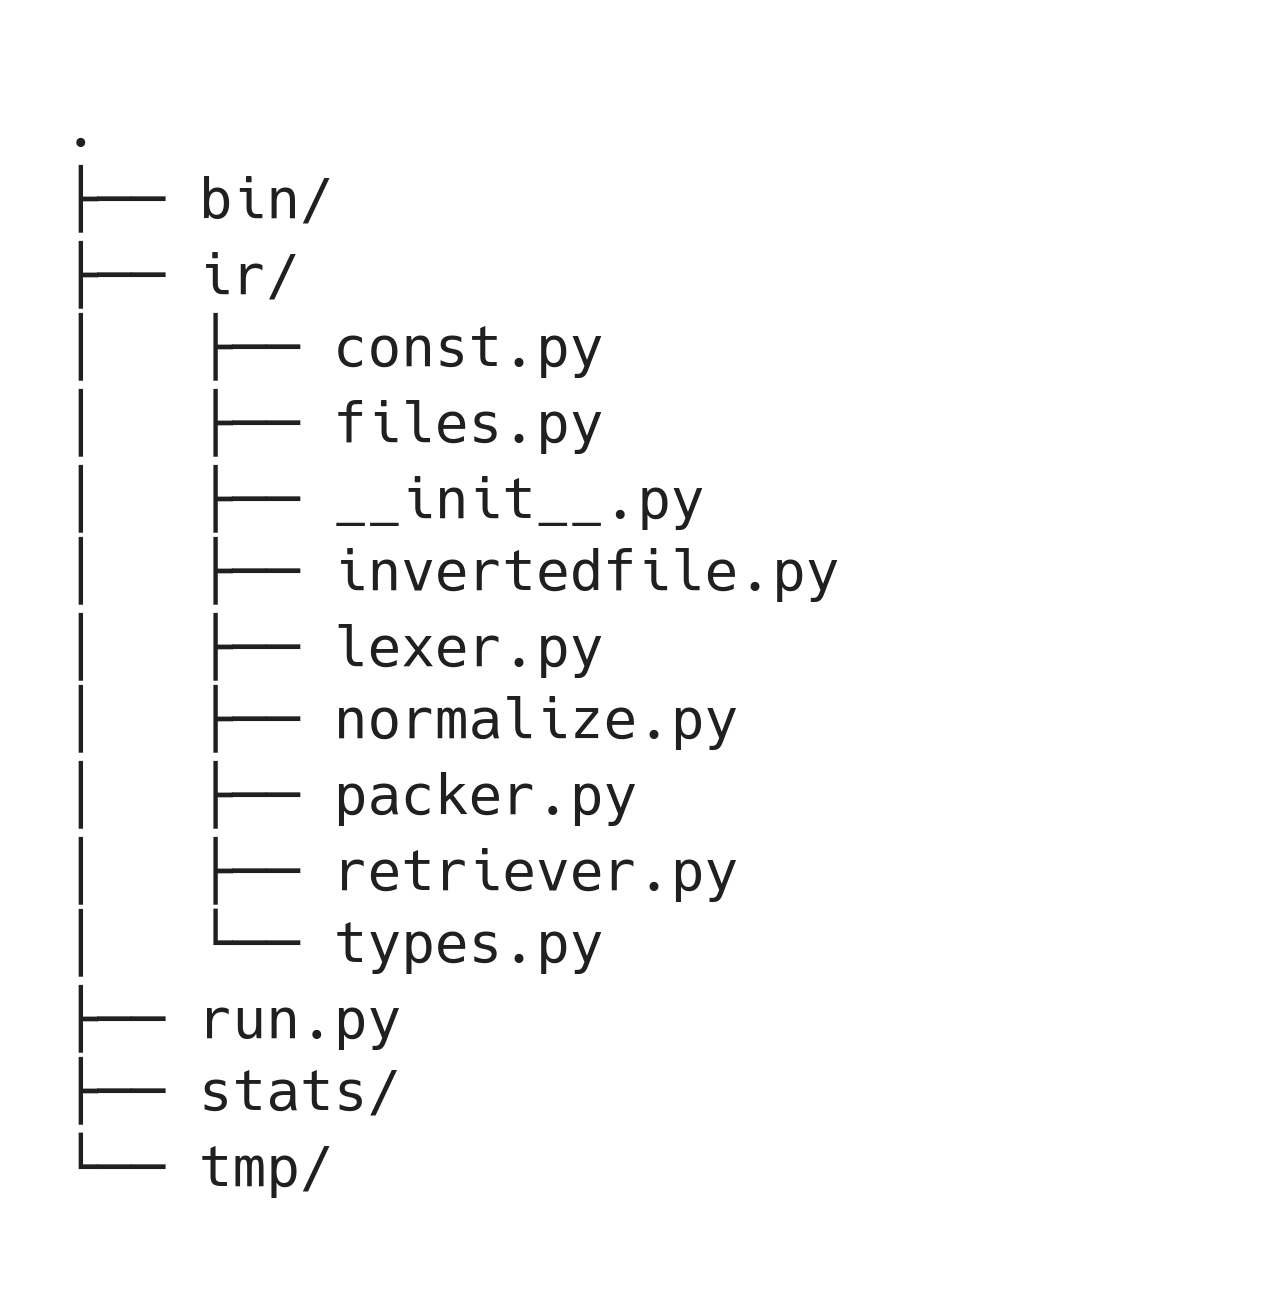
\includegraphics[scale=0.2]{statics/dirtree.png}
    \caption{Directory Hierarchy of Assignment 3}
\end{figure}

The source code for all of the files are attached in Appendix \ref{appendix:src}.

The total number of non-empty lines of code for the program totals to under 750.

\begin{figure}[!ht]
    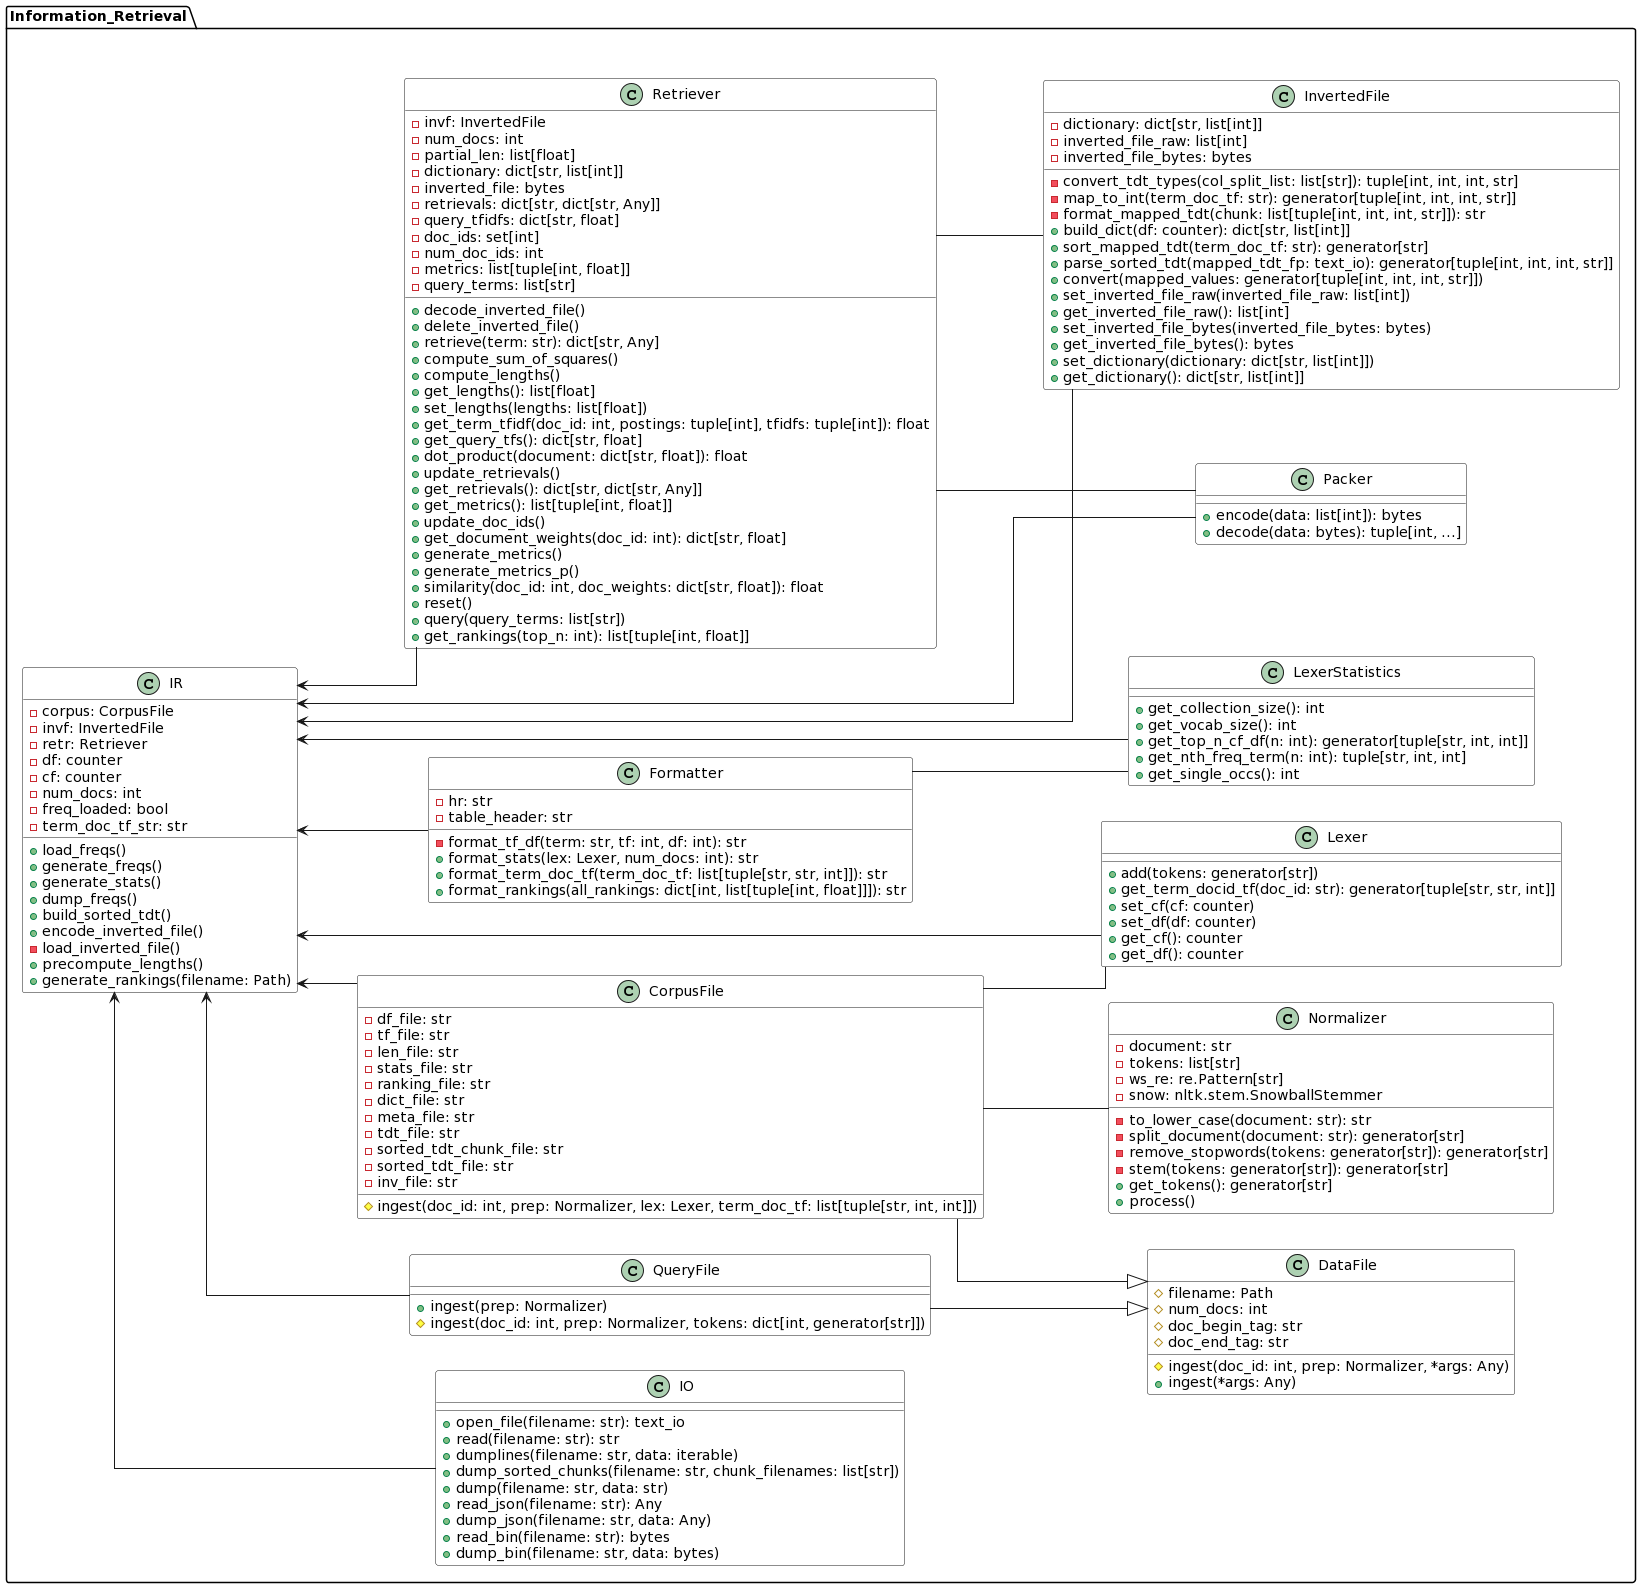
\includegraphics[scale=0.31]{statics/uml.png}
    \centering
    \caption{UML of Information Retrieval}
\end{figure}

\subsection{Existing Classes}

\subsubsection{Driver} \label{sec:driver}
The driver script for the program is \texttt{run.py}. The script uses command line options to process corpus files to perform the following operations:

\begin{enumerate}
    \item generate document and relative term frequencies
    \item generate statistics on corpus frequencies
    \item save frequencies to file
    \item extract term-docID-term frequency records and save to temporary files
    \item generate, encode and save inverted file
    \item compute document weights and save for repeated use
    \item process query files and generate rankings
\end{enumerate}

\subsubsection{\texttt{lexer.Lexer}}
The \texttt{Lexer} class had its methods on generating statistics separated into the \texttt{LexerStatistics} class.

\subsubsection{\texttt{files} Classes}
The \texttt{DataFile} class was renamed to \texttt{CorpusFile} and the \texttt{QueryFile} class was added to ingest query files. Both of these classes have been derived from the \texttt{DataFile} class.

The \texttt{Formatter} class has a new method to format rankings.

The \texttt{IO} class has a new method for writing chunks of data to files to be merged again. This method is only used for dumping chunks of sorted term-docID-term frequency records.

\subsubsection{\texttt{invertedfile.InvertedFile}}
The \texttt{InvertedFile} class received the following modifications:
\begin{itemize}
    \item the dictionary now only contains the term index, offset, length, and document frequency for each terms.
    \item the term-docID-term frequency records were sorted and saved to files in chunks. The chunk files are later merged to a single sorted file. This approach allows for the program to process  large corpuses without stressing the memory.
\end{itemize}

\subsection{\texttt{New Classes}}

\subsubsection{\texttt{retriever.Retriever}}
The\texttt{Retriever} class was added to compute document weights and rank queries.

The class precomputes document weights to save to a file for repeated use.


\section{Statistics and Observations}
With the modifications made to the text normalization process, the statistics generated from the input file have changed. The new top 10 more frequent tokens now include "market", "announc", and "report", which are terms that expected in headlines.

In terms of the inverted files and dictionaries, the space they occupy on disk combined are significantly lower than the original document.

\begin{table}[h]
    \begin{center}
        
        \begin{tabular}{| l | r | l |}
        \hline
        \textbf{File} & \textbf{Size (in bytes)} & \textbf{Description} \\
        \hline
        headlines.txt & 39381610 & Input corpus file \\
        headlines\_dict.json & 4275427 & Generated dictionary JSON file \\
        headlines\_if.bin & 27774312 & Inverted binary file \\
        \hline
        \end{tabular}

    \end{center}
    \caption{Sizes of Files Computed Through the \texttt{stat} Command on a Debian Based Linux}

\end{table}

\section{Testing}
The tests described by the prompt were performed via the \texttt{test.py} driver script. The tokens to look up had to first be normalized through the \texttt{Normalizer} class.

\begin{lstlisting}[style=mypython,
    caption=Test 1: Document frequency and postings list for the terms: "Heidelberg"\, "cesium"\, "Trondheim"\, "crustacean"]
# NOTE: the normalization stems "crustacean" to "crustacea"
# and "crustaceans" to "crustacean"
tokens1 = normalize_test_terms(
    prep, ("Heidelberg", "cesium", "Trondheim", "crustaceans")
)
results1 = read_inverted_file(
    invf,
    tokens1,
    ("term", "postings", "postings_len"),
)
\end{lstlisting}

% \begin{figure}[!ht]
%     \centering
%     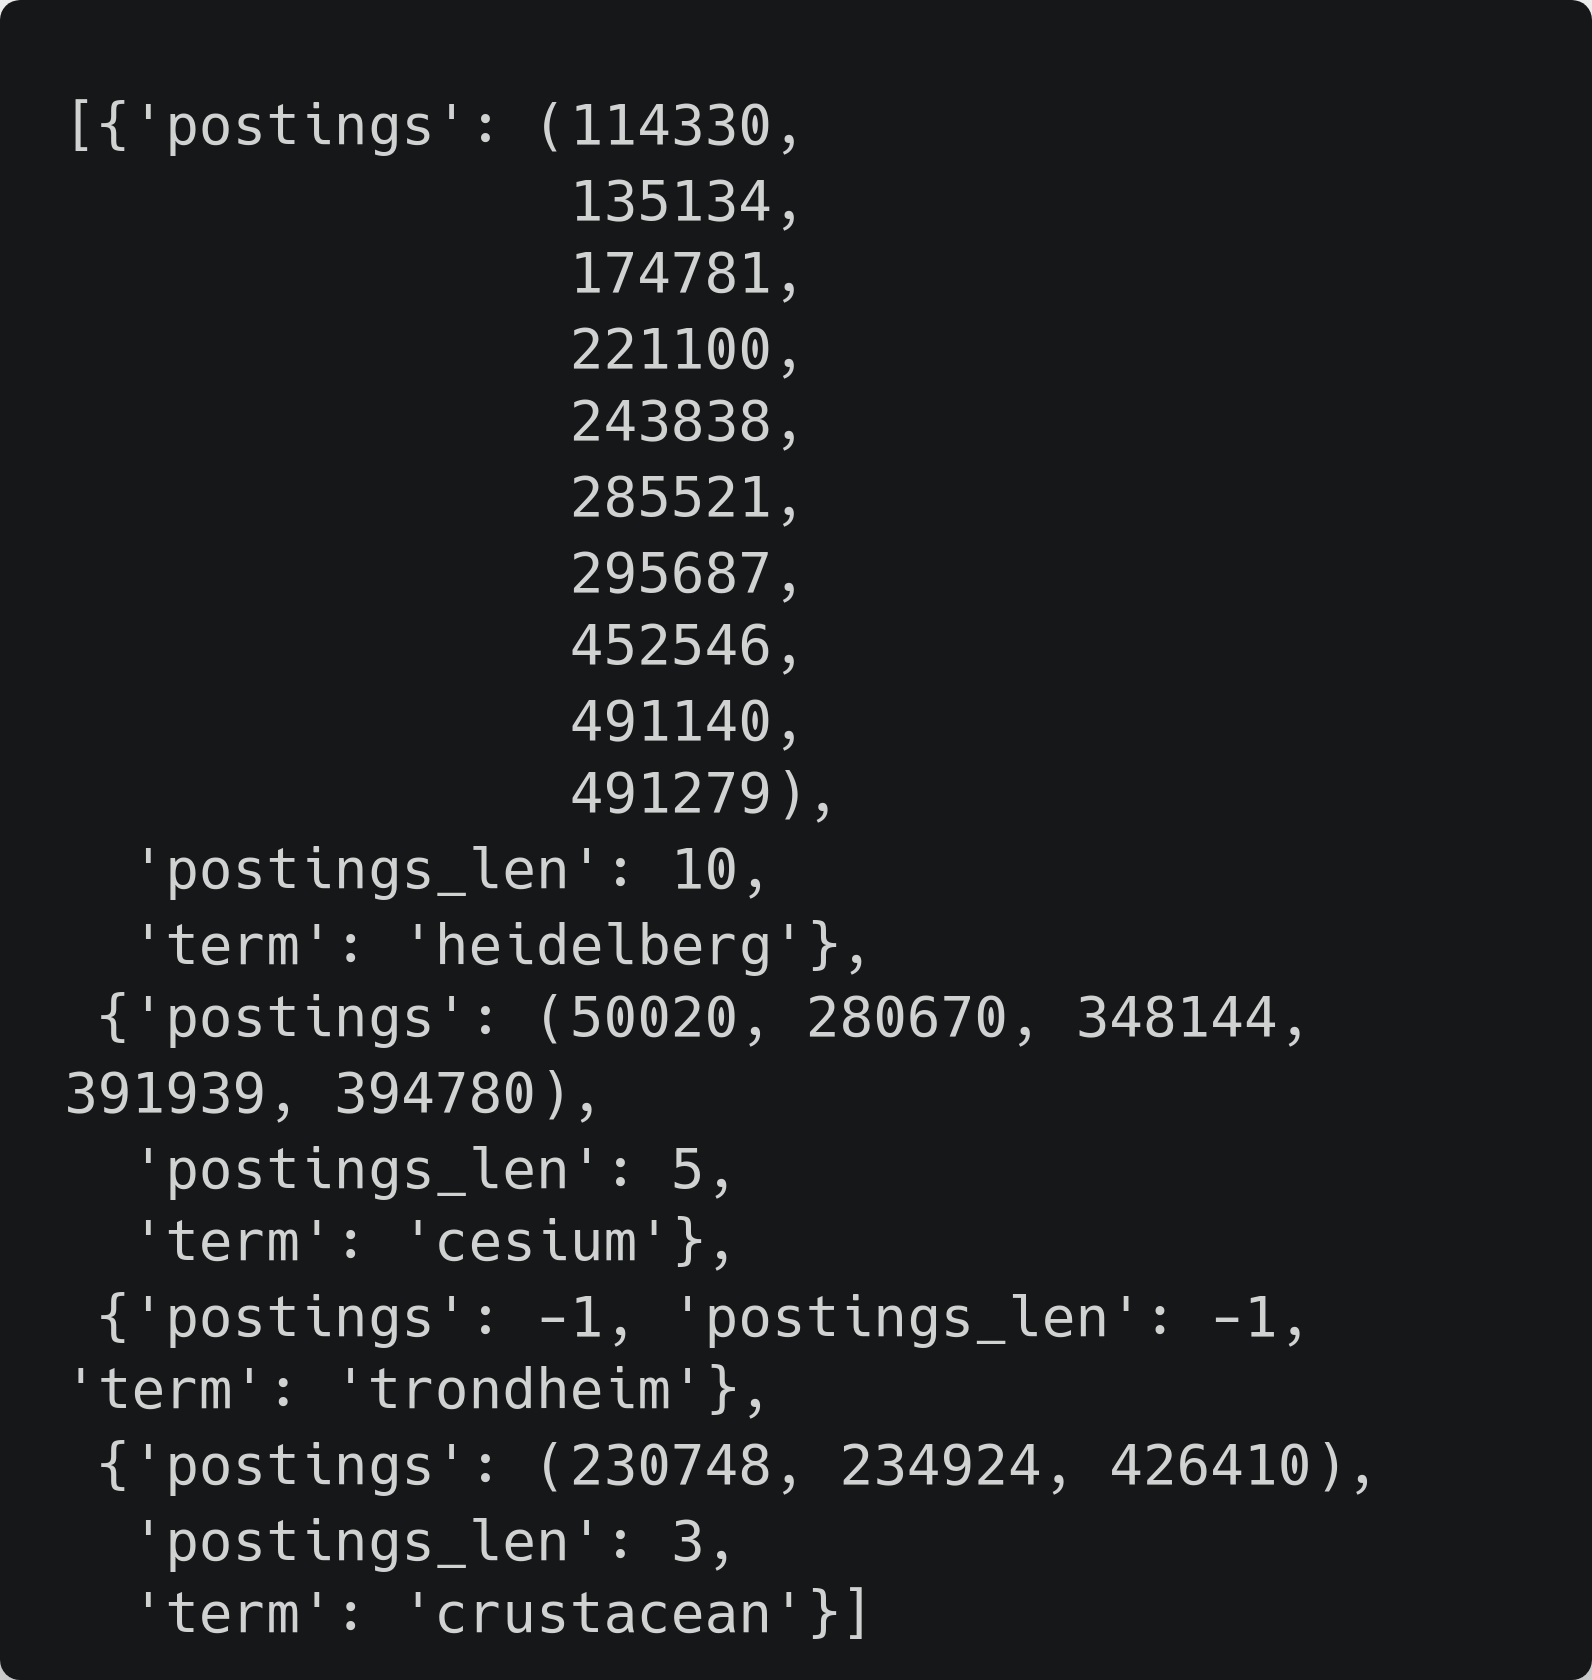
\includegraphics[scale=0.15]{statics/test1.png}
%     \caption{Output of Test 1}
% \end{figure}
% \clearpage
% \newpage

\begin{lstlisting}[style=mypython,caption=Test 2: Document frequency for the words: "Hopkins"\, "Stanford"\, "Brown"\, and "college"]
tokens2 = normalize_test_terms(
    prep, ("Hopkins", "Stanford", "Brown", "college")
)
results2 = read_inverted_file(invf, tokens2, ("term", "postings_len"))
\end{lstlisting}
% \clearpage
% \newpage

% \begin{figure}[!ht]
%     \centering
%     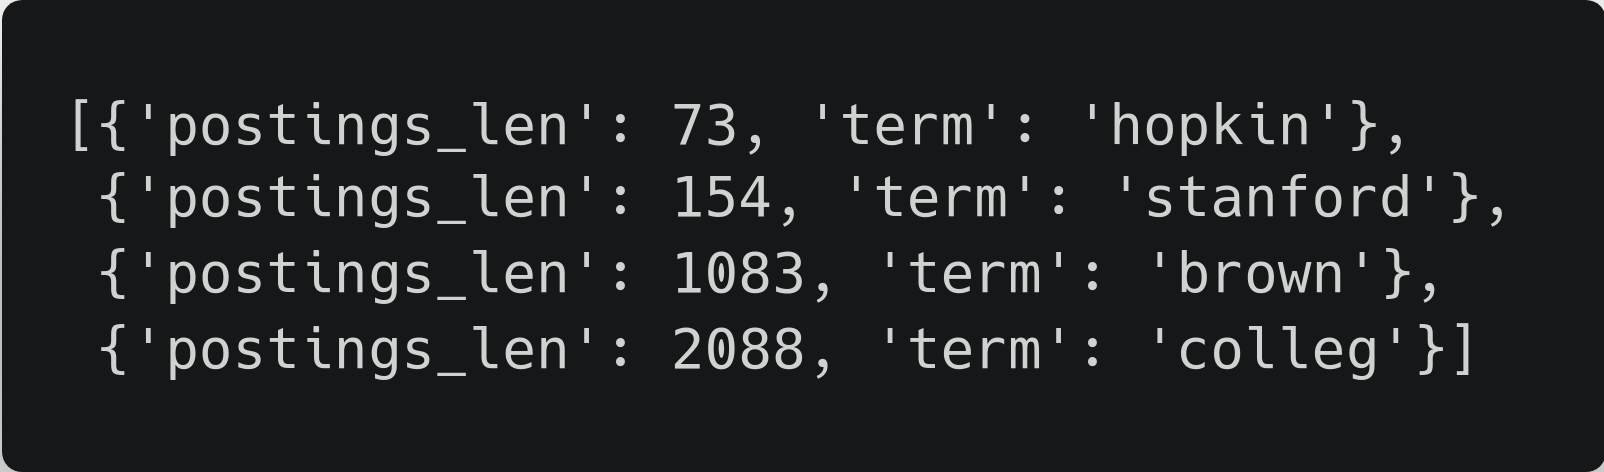
\includegraphics[scale=0.15]{statics/test2.png}
%     \caption{Output of Test 2}
% \end{figure}

\begin{lstlisting}[style=mypython,caption=Test 3: docids for documents that have both "Elon" and "Musk"]
# NOTE: the normalization stems "Musks" to "Musk"
tokens3 = normalize_test_terms(prep, ("Elon", "Musks"))
results3 = read_inverted_file(invf, tokens3, ("postings",))
elon, musk = results3
elon_postings, musk_postings = set(elon["postings"]), set(musk["postings"])
elon_musk_postings = elon_postings & musk_postings
\end{lstlisting}

% \begin{figure}[!ht]
%     \centering
%     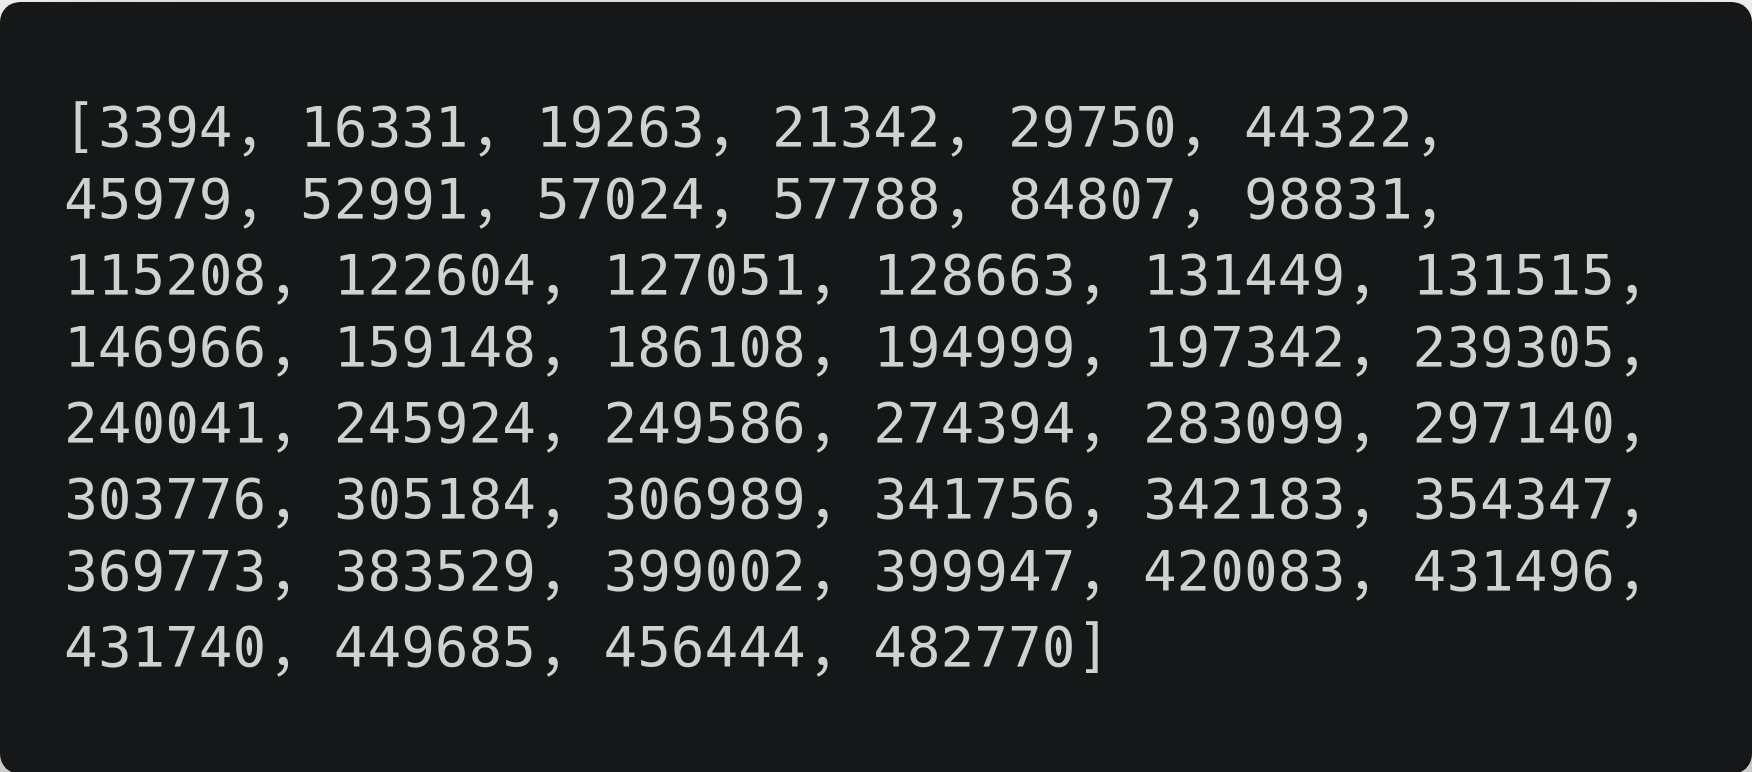
\includegraphics[scale=0.15]{statics/test3.png}
%     \caption{Output of Test 3}
% \end{figure}

\appendix

\section{Source Code} \label{appendix:src}

\inputpython{../ir/const.py}{../ir/const.py}
\inputpython{../ir/files.py}{../ir/files.py}
\inputpython{../ir/invertedfile.py}{../ir/invertedfile.py}
\inputpython{../ir/lexer.py}{../ir/lexer.py}
\inputpython{../ir/normalize.py}{../ir/normalize.py}
\inputpython{../ir/packer.py}{../ir/packer.py}
\inputpython{../ir/retriever.py}{../ir/retriever.py}
\inputpython{../ir/types.py}{../ir/types.py}

\inputpython{../run.py}{../run.py}

\section{Outputs} \label{appendix:outputs}

\lstinputlisting[caption=Statistics of 'cord19.txt',basicstyle=\small]{../outputs/stats/cord19_summary.txt}

\end{document}
